\section{Zeitauswertung}

\subsection{Zweck dieses Dokuments}
Die Zeitauswertung zeigt auf, wann und wo wieviel Zeit aufgewendet wurde. Dabei haben wir drei unterschiedliche Auswertungen angefertigt, welche in den nachfolgenden Unterkapitel genauer erläutert werden.

\subsection{Zeitliche Auswertung nach Monaten}
Die erste Auswertung zeit die aufgewendete Zeit nach Monaten. 
Während den fünf Monaten, in denen das Projekt lief, haben wir insgesamt 724.5 Stunden aufgewendet. Dies entspricht ziemlich genau dem Richtwert von 720 Stunden. 
Da das Projekt am 18. Februar 2019 startete, fallen die 77 Stunden, welche im Februar geleistet wurden, etwas geringer aus als in den restlichen Monaten. In den Monaten März, April und Mai wurden gesamthaft 185 Stunden, 175 Stunden bzw. 202 Stunden investiert. Im Juni gingen die aufgewendeten Stunden wieder auf ca. 84 Stunden zurück, da das Projektende Mitte Monat (14. Juni 2019) war.

\begin{figure}[h]
  \centering
  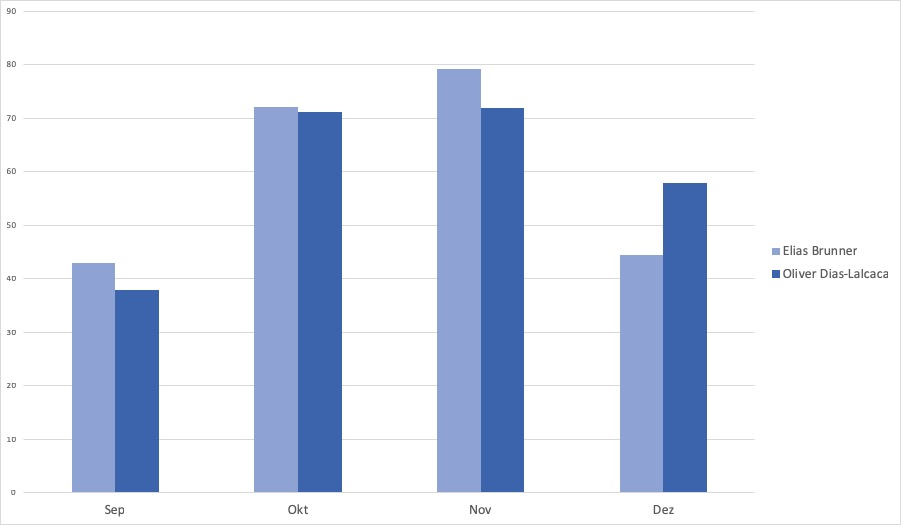
\includegraphics[width=1\linewidth]{./img/zeitauswertung/ZeitauswertungMonate}
  \caption{Zeitliche Auswertung nach Monaten}
  \label{fig:comparison-month}
\end{figure}

\subsection{Zeitliche Auswertung nach Sprints}
Die Zeitauswertung anhand der durchgeführten Sprints zeigt wie viel Zeit in den einzelnen Sprints investiert wurden.

Dabei ist zu beachten, dass wir einzelne Tickets teilweise über mehrere Sprints bearbeiteten. Meistens geschah dies, weil wir mit dem Ticket noch nicht fertig waren.

Die Auswertung zeigt daher nicht nur die definierten Sprints bzw. die Zeiten, die in jenem Sprint geleistet wurden, sondern auch den oben erwähnten Fall.

Der Ausreisser von 83.25 Stunden ist dadurch zu erklären, dass es sich dabei hauptsächlich um die Arbeiten des Refactorings (siehe Anhang \ref{sec:code-review}) handelt und wir dabei generell mehr Zeit benötigten als zunächst gedacht. Im Speziellen für das Frontend, was Oliver Dias-Lalcaca übernommen hat.

\begin{figure}[h]
  \centering
  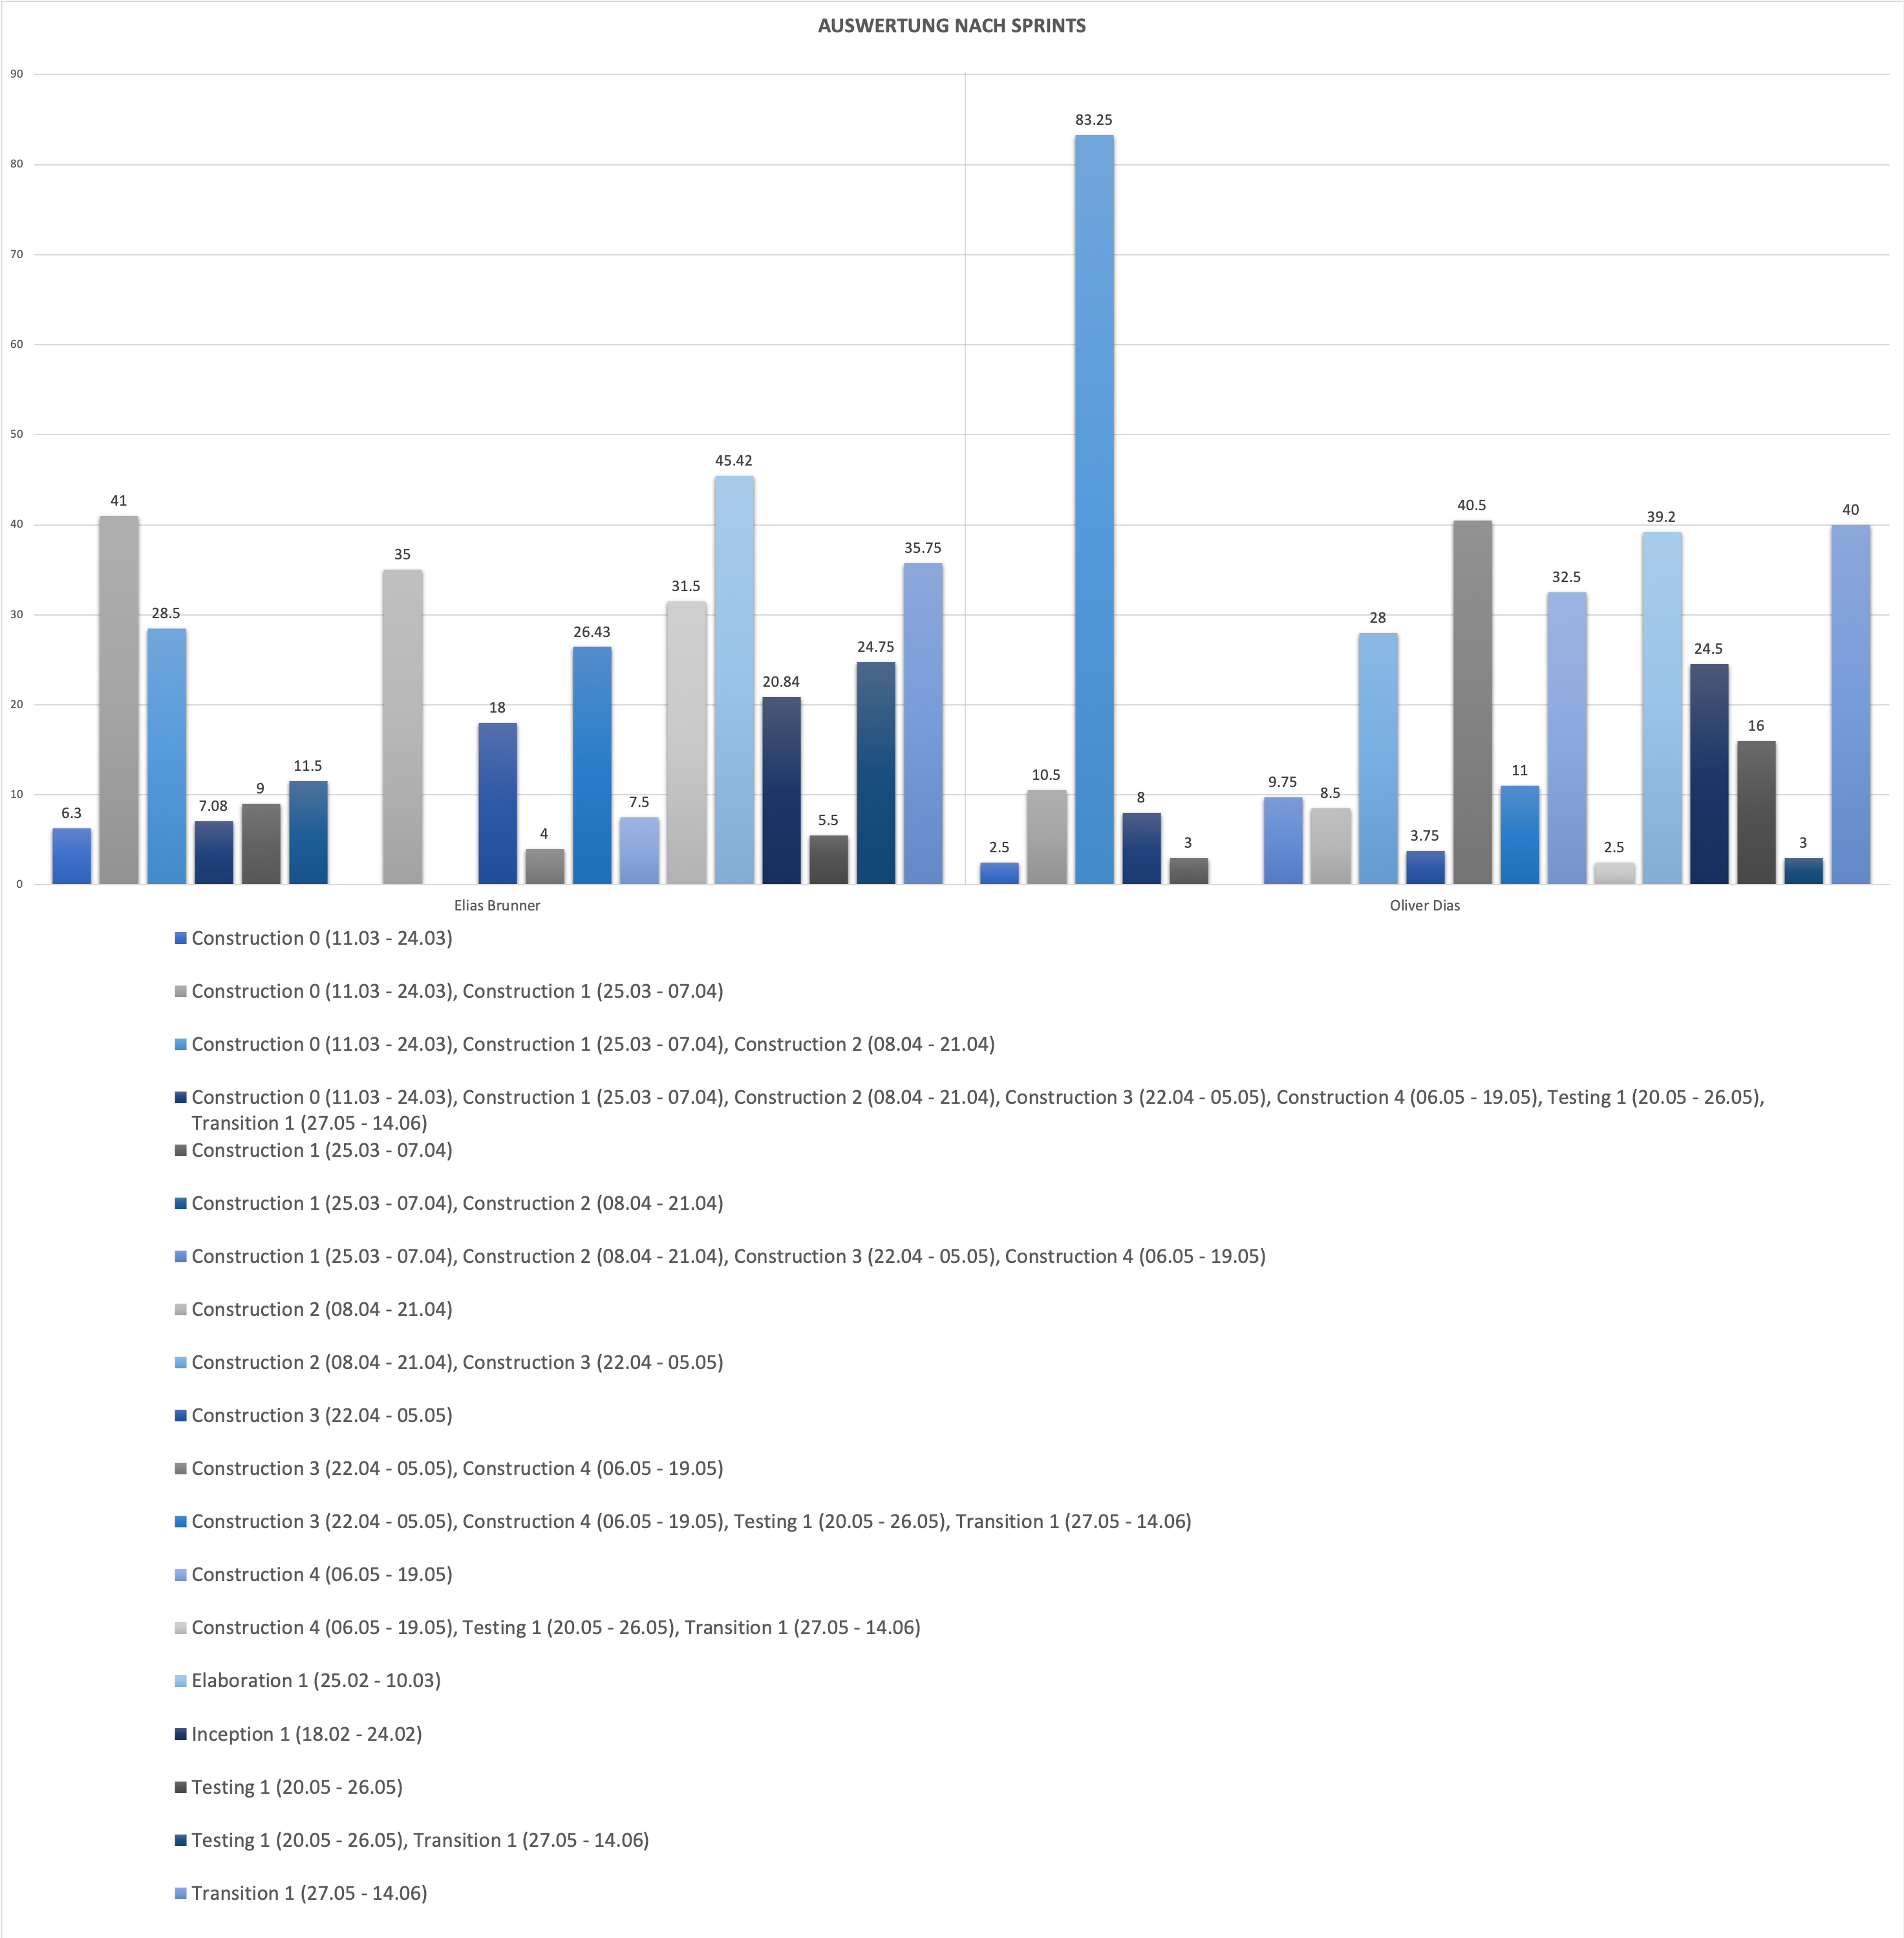
\includegraphics[width=1\linewidth, height=15cm]{./img/zeitauswertung/ZeitauswertungSprints}
  \caption{Zeitliche Auswertung nach Sprints}
  \label{fig:comparison-sprints}
\end{figure}

\subsection{Zeitliche Auswertung nach Arbeitskategorien}
Zuletzt interessierte uns noch wie viel Zeit wir für die einzelnen Arbeitskategorien (Labels) aufgewendet haben.

Um das Diagramm zu verstehen muss gesagt werden, dass der innere Kreis die Zeiten für Elias Brunner repräsentiert und der äussere Kreis die Zeiten für Oliver Dias-Lalcaca darstellt. 

Die prozentuale Aussage gibt ein ungefähren Überblick über die investierten Zeiten für die einzelnen Arbeitskategorien. Dabei fällt auf, dass wir die meiste Zeit in die Entwicklung 34 \% bzw. 64\% (durchschnittlich 49\%) und die Dokumentation 29\% bzw. 14\% (durchschnittlich 21\%) investiert haben.

\begin{figure}[h]
	\centering
	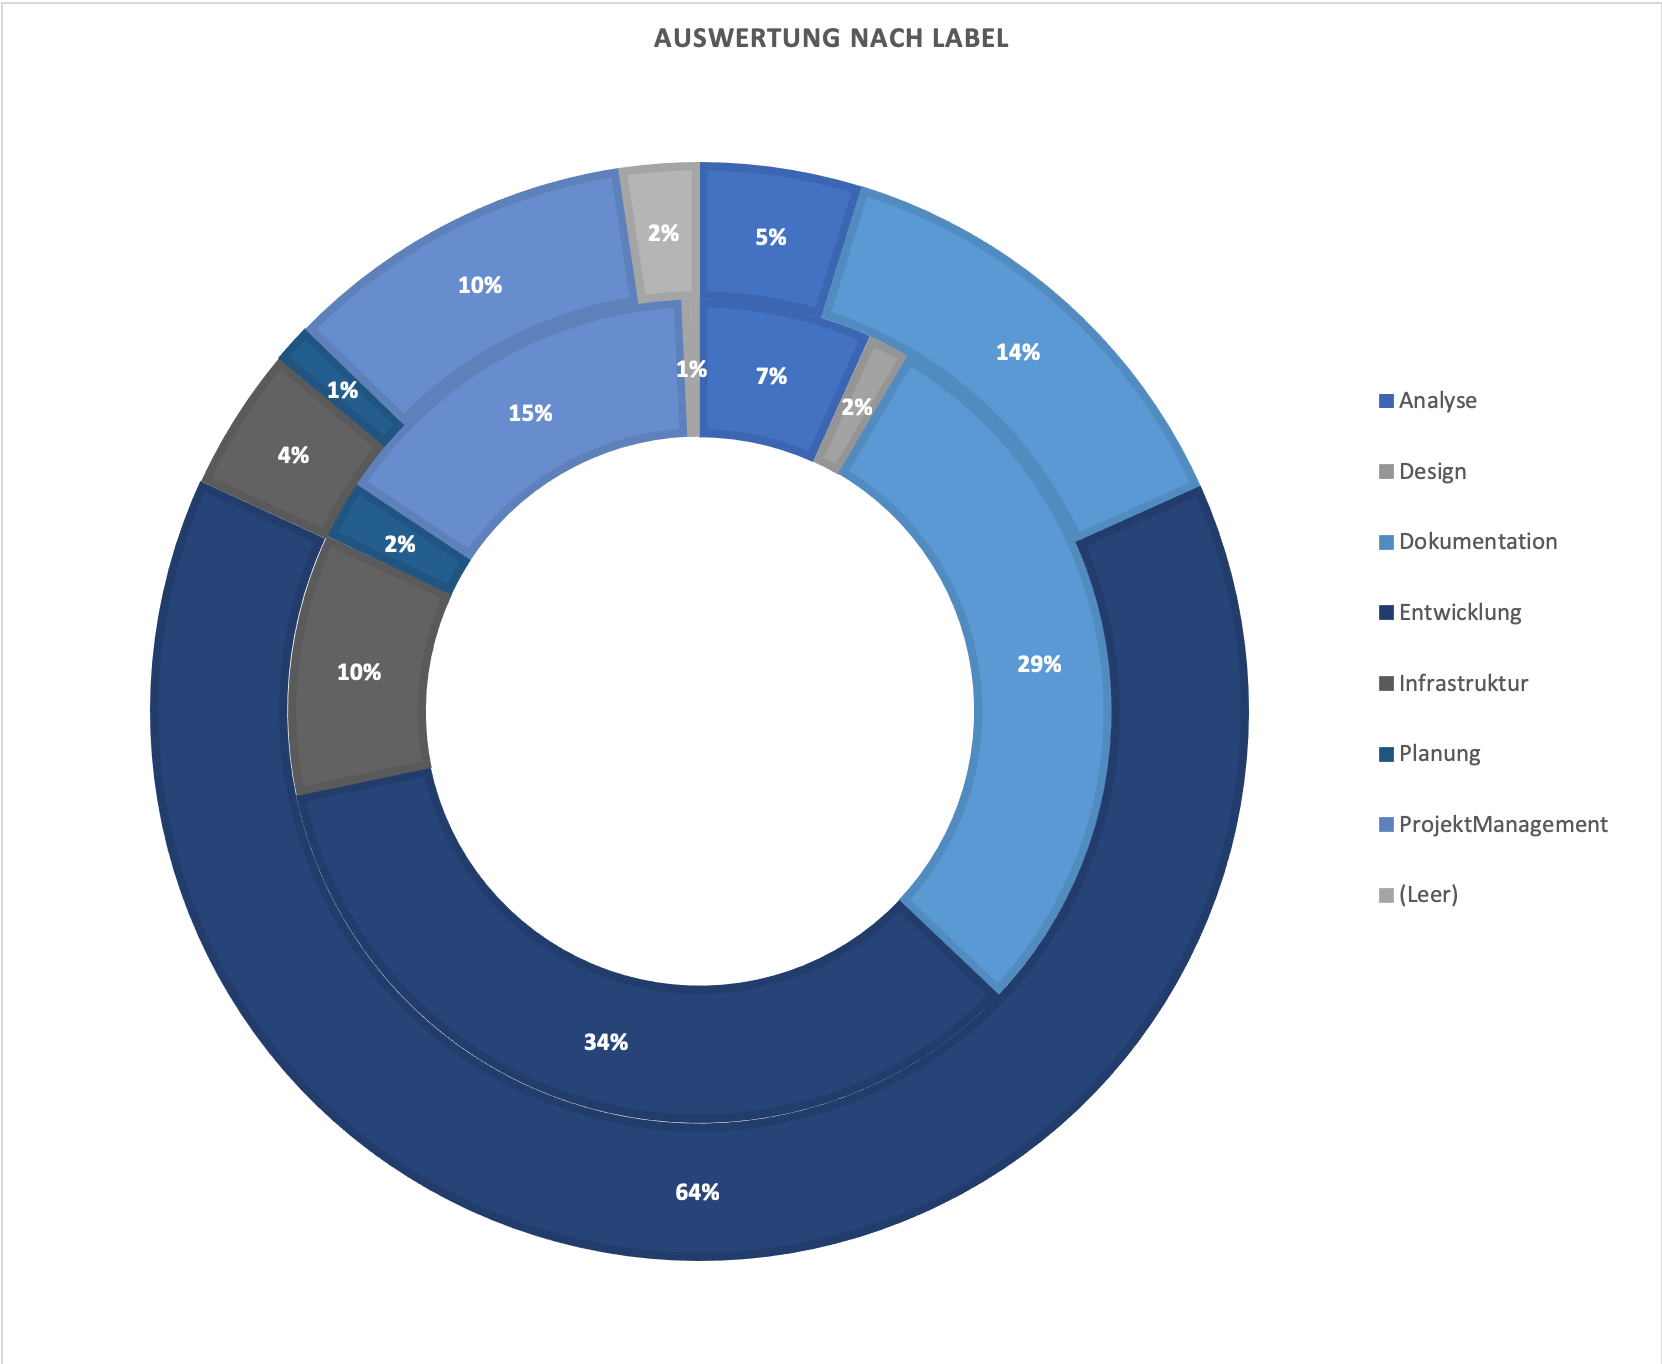
\includegraphics[width=1\linewidth]{./img/zeitauswertung/ZeitauswertungLabel}
	\caption{Zeitliche Auswertung nach Labels}
	\label{fig:comparison-labels}
\end{figure}